\documentclass{article}
\usepackage[utf8]{inputenc}
\usepackage{amsmath}
\usepackage{mathtools}
\usepackage{graphicx}

\title{Stats Template}
\author{Carlyle Morgan}
\date{May 2021}
\graphicspath{{../ImageFiles}}


\begin{document}


    \section{Luxburg: A Tutorial on Spectral Clustering}

        \subsection{Basics of Graph Theory}
            A \textbf{similarity graph} (say $G = (V,E)$) is a form of representing the similarities between points in a dataset ($x_1, x_2, ..., x_n)$, with $s_{ij}$, some measure of similarity between two points weighting the E edges between V vertices. Each vertex in this graph corresponds to a data point in $X$. These vertices are connected if the measure of similarity between the data points they represent exceeds some arbitrary threshold. 
    Some helpful terms to remember:
            \begin{itemize}
                \item A \textbf{weight} of an edge is some arbitrary non-negative value assigned to that edge. 
                \item An \textbf{adjacency matrix},  is the matrix form of denoting whether two vertices are connected, taking values of 1 if the vertices are connected and 0 if not. For example, if 1 is connected to 2 and 2 is connected to 3, adjacency matrix $A_{ij} $ is:
                        $$A_{ij} = \begin{bmatrix}
                0 & 1 & 0\\
                1 & 0 & 1\\
                0 & 1 & 0
                \end{bmatrix}$$
                A \textbf{weighted adjacency matrix} (typically denoted $W_{ij}$) is the matrix such that instead of taking the values 0 and 1, each element of the matrix takes the value of the edge weight instead.
                \item The \textbf{degree} of a vertex is the sum of the weights of edges connected to that vertex. This information can be summarized in a \textbf{degree matrix}, $D$, a diagonal matrix where the degrees of each vertex form the diagonal entries of the matrix. 
                \end{itemize}
    There are multiple ways to measure the "size" of a subset of the verticies in G. For arbitrary $A \subset V$:
    
\begin{enumerate}
\item  $\left|A\right|$ measures the size of A by the number of vertices in A
\item vol($A$) measures the size of A by the sum of all weights attached to vertices in A
\end{enumerate}

When dealing with subsets of graphs, it is helpful to know the following terms:
\begin{itemize}
\item A subset of vertices is \textbf{connected} if any two vertices in that subset can be joined by a path such that all intermediate points lie in that subset.
\item A subset of vertices is a \textbf{connected component} if it is connected and there are no connections to vertices outside the subset.
\end{itemize}

\subsection{Graph Laplacians}

Spectral graph theory is the study of \textbf{graph Laplacians}, matricies containing important information about the graph being studied. No one necessarily agrees how one should define the Laplacian matrix, but how you choose to do it will determine what information you are considering about the graph when you perform clustering. That being said, there are a few commonly used definitions already in the literature:
\begin{enumerate}
\item  The unnormalized graph Laplacian is defined such that: $$ L = D - W$$ with $D$ and $W$ being the degree and weighted adjacency matrix. This definition of the Laplacian has a nice property such that the multiplicity of the eigenvalue 0 for this matrix is equivalent to the number of connected components in the graph of interest. 

\item The normalized symmetric graph Laplacian is defined such that: $$ L = I - D^{-1/2}WD^{-1/2}$$
The normalized random walk graph Laplacian is defined such that: $$ L = I - D^{-1}W$$



These definitions of the Laplacian also exhibit the nice property of the unnormalized Graph Laplacian. However, the eigenspace of 0 is spanned by the indicator vector for the normalized random walk graph Laplacian and $D^{1/2}$ times the indicator vector for the normalized symmetric graph Laplacian.

\end{enumerate}

\subsection{Spectral Clustering}

\subsubsection{Intuition}

Say we wish to cluster the different data points in $X$ into different groups according to their similarities. In other words, we wish to divide up the graph into sections such that the edges between sections have low weight. 

To accomplish this, we first need to define the concept of a cut. For some subset $A \subset V$, $\bar A = V / A$.

$$\text{cut}(A_1,...,A_k):=\frac{1}{2}\sum_{i=1}^{k}W(A_i,\bar A_i)$$

This simply reads that we are summing the weights of all edges between A and not A for all possible partitions of A, and then halving this sum to not double count. Grouping the vertices into $(A_1,...,A_k)$ such that $\text{cut}(A_1,...,A_k)$ thus achieves the desired result. However, in practice this often only results in one vertex being separated from the rest of the graph. Thus, one applies weighting such that each $A_i$ must instead be reasonably large. There are two common ways to achieve this weighting, RatioCut and NCut:

\begin{itemize}
\item Ratiocut weights the cut but dividing by $\left|A\right|$, the number of edges in A for each $A_i$
\item Ncut weights the cut but dividing by $\text{vol}(A_i)$, the sum of the weight of edges in A for each $A_i$
\end{itemize}

Just like for the unweighted case, a good partion will minimize Ratiocut or Ncut. Both these techniques result in "balanced" (according to their objective function) groups for each $A_i$. Adding these weights will melt your computer, as they are very computationally intensive. An approximate, less intensive method is needed.

It turns out that Ratiocut can be reasonably approximated for any number of desired partitions by a manipulation of the unnormalized graph Laplacian. Likewise, Ncut can be reasonably approximated for any number of desired partitions by a manipulation of the normalized graph Laplacian.

\subsubsection{Popular Spectral Clustering Methods}
These manipulations are the spectral clustering algorithms, a few of which are the following:

\begin{figure}
  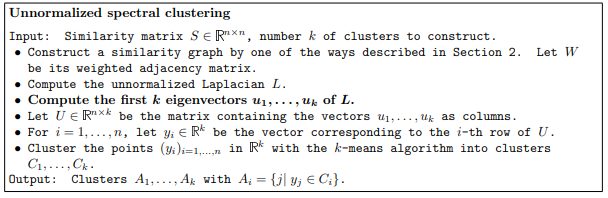
\includegraphics[width=\linewidth]{unnormsc.PNG}
  \caption{A boat.}
  \label{fig:boat1}
\end{figure}

\subsubsection{Random Walks and Clustering on Probability}

Instead of clustering on some property of cuts, instead say that we wish to cluster on the basis of probability. We wish to partition our graph such that a random walk will spend a lot of time in a certain cluster before moving to the next. Simply define the transition probability from one state to the next to be proportional to the weight of the edge between two vertices. A transition matrix of these probabilities is: $$P = D^{-1}W$$, which looks very similar to how we defined the normalized symmetric graph Laplacian, as $L_{rw} = I - D^{-1}W = I -P$. Our strategy for clustering based on this matrix is similar to that for graph Laplacians, where we simply compute the eigenvectors to determine cluster properties of this graph. 

Shi and Malik(2001) prove that though we did not even think about any sort of measure like Ncut or Ratiocut, the transition probabilities of a random walk on our graph and Ncut are equivalent. Thus, the normalized spectral clustering algorithm we used to approximate Ncut also produces results that minimize transition probabilities outside of certain clusters. The symmetric normalized graph Laplacian can also be used for find commute distances, the expected time it takes the random walk to travel between any two vertices and back.

\subsubsection{Perturbation Theory}

Perturbation theory studies how eigenvalues and eigenvectors of a matrix change under the presence of some small perturbation. For some original matrix $A$, consider some perturbation matrix $H$. Thus, the perturbed matrix, $A_p$ is $A_p = A + H$.  Observed network data can be seen as $A_p$, and the object of our analysis is to work the matrix back to $A$, where $A$ contains the "true" communities in the data with minimal connections outside of these communities. This provides the framework for a different conceptual approach to the clustering process.


            
\end{document}
